\chapter{Formal Analysis Using Alloy}
In this chapter the Alloy model of the eMall system is implemented, describing the main constraints and focusing in particular on the consistency of the world.\\
For this purpose, 2 different sub-worlds are created which allow you to view their characteristics.
\lstinputlisting[language=alloy]{alloy/eMall.als}
\clearpage
\begin{figure}[H]
\centering
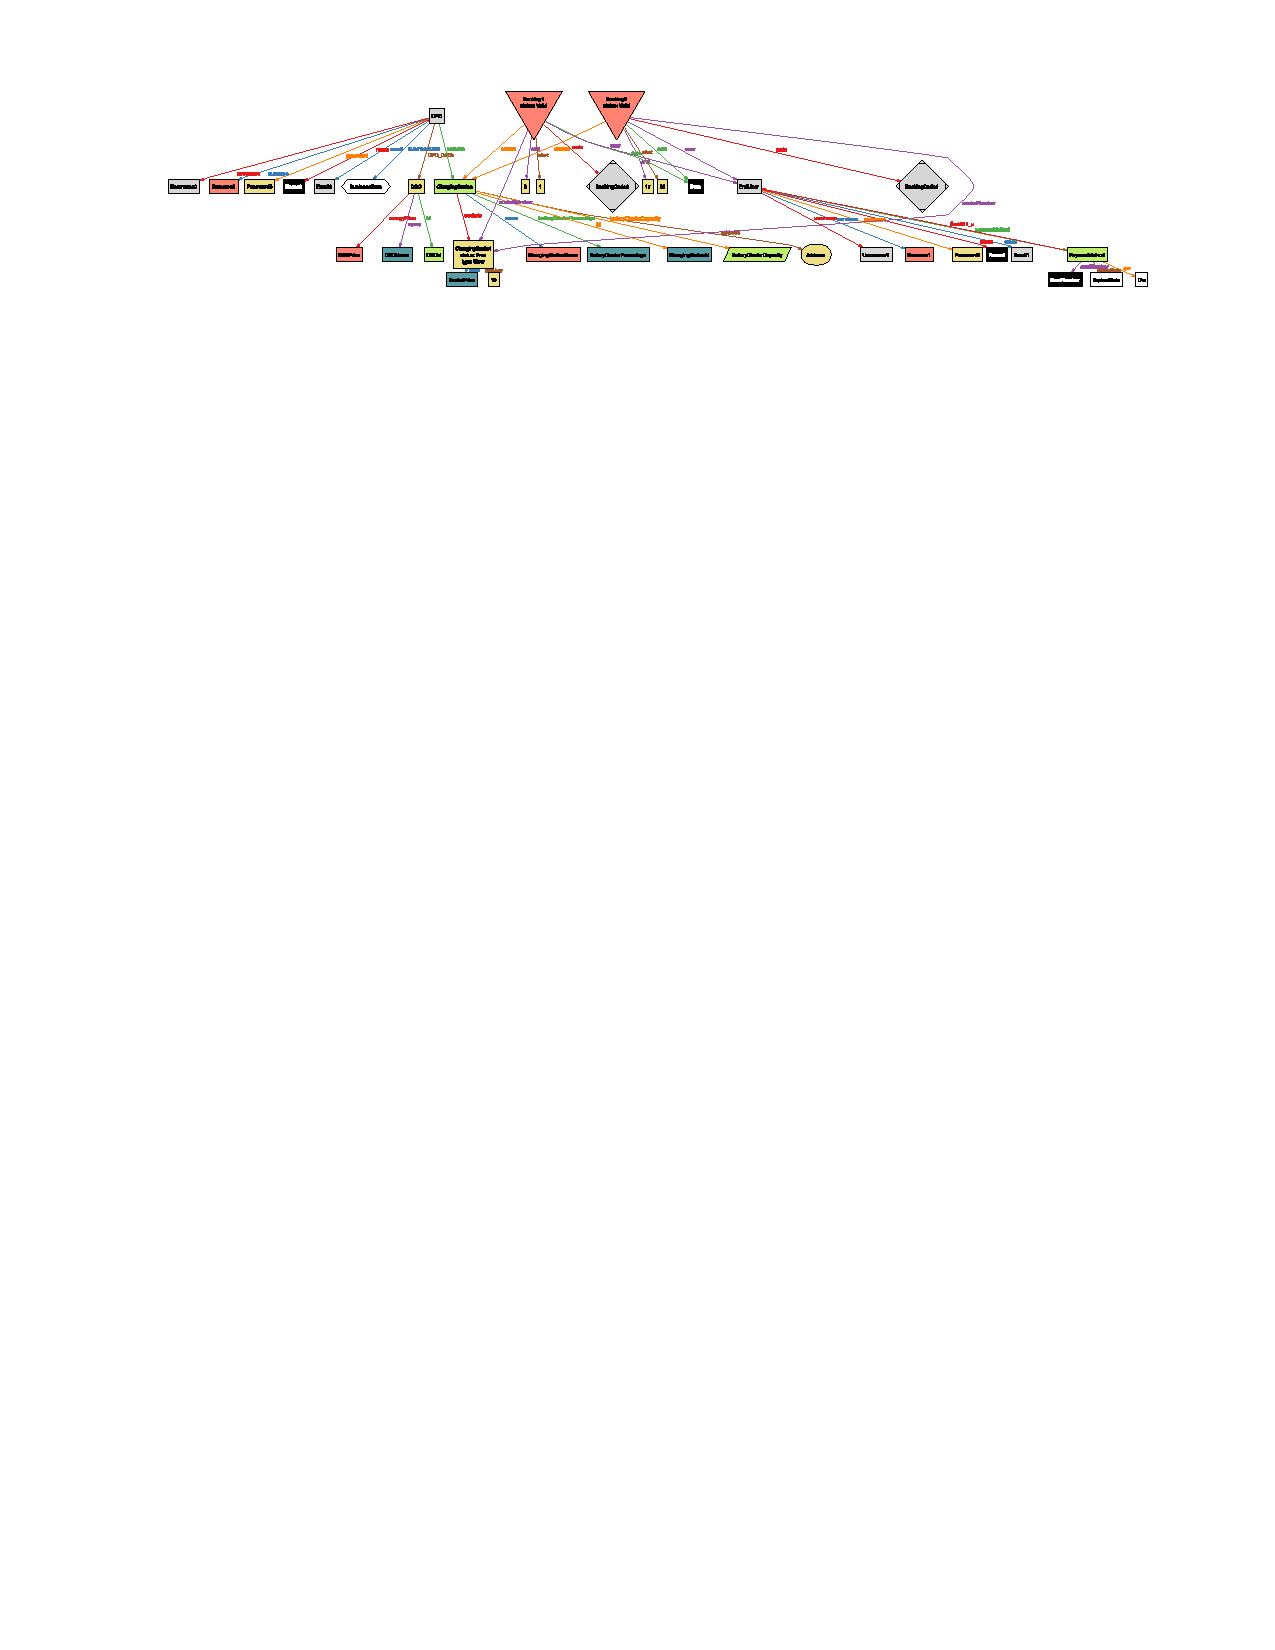
\includegraphics[angle=90,origin=c, height=0.85\textwidth]{images/world1.pdf}
\caption{World 1}
\label{fig:world_1}
\end{figure}
\begin{figure}[H]
\centering
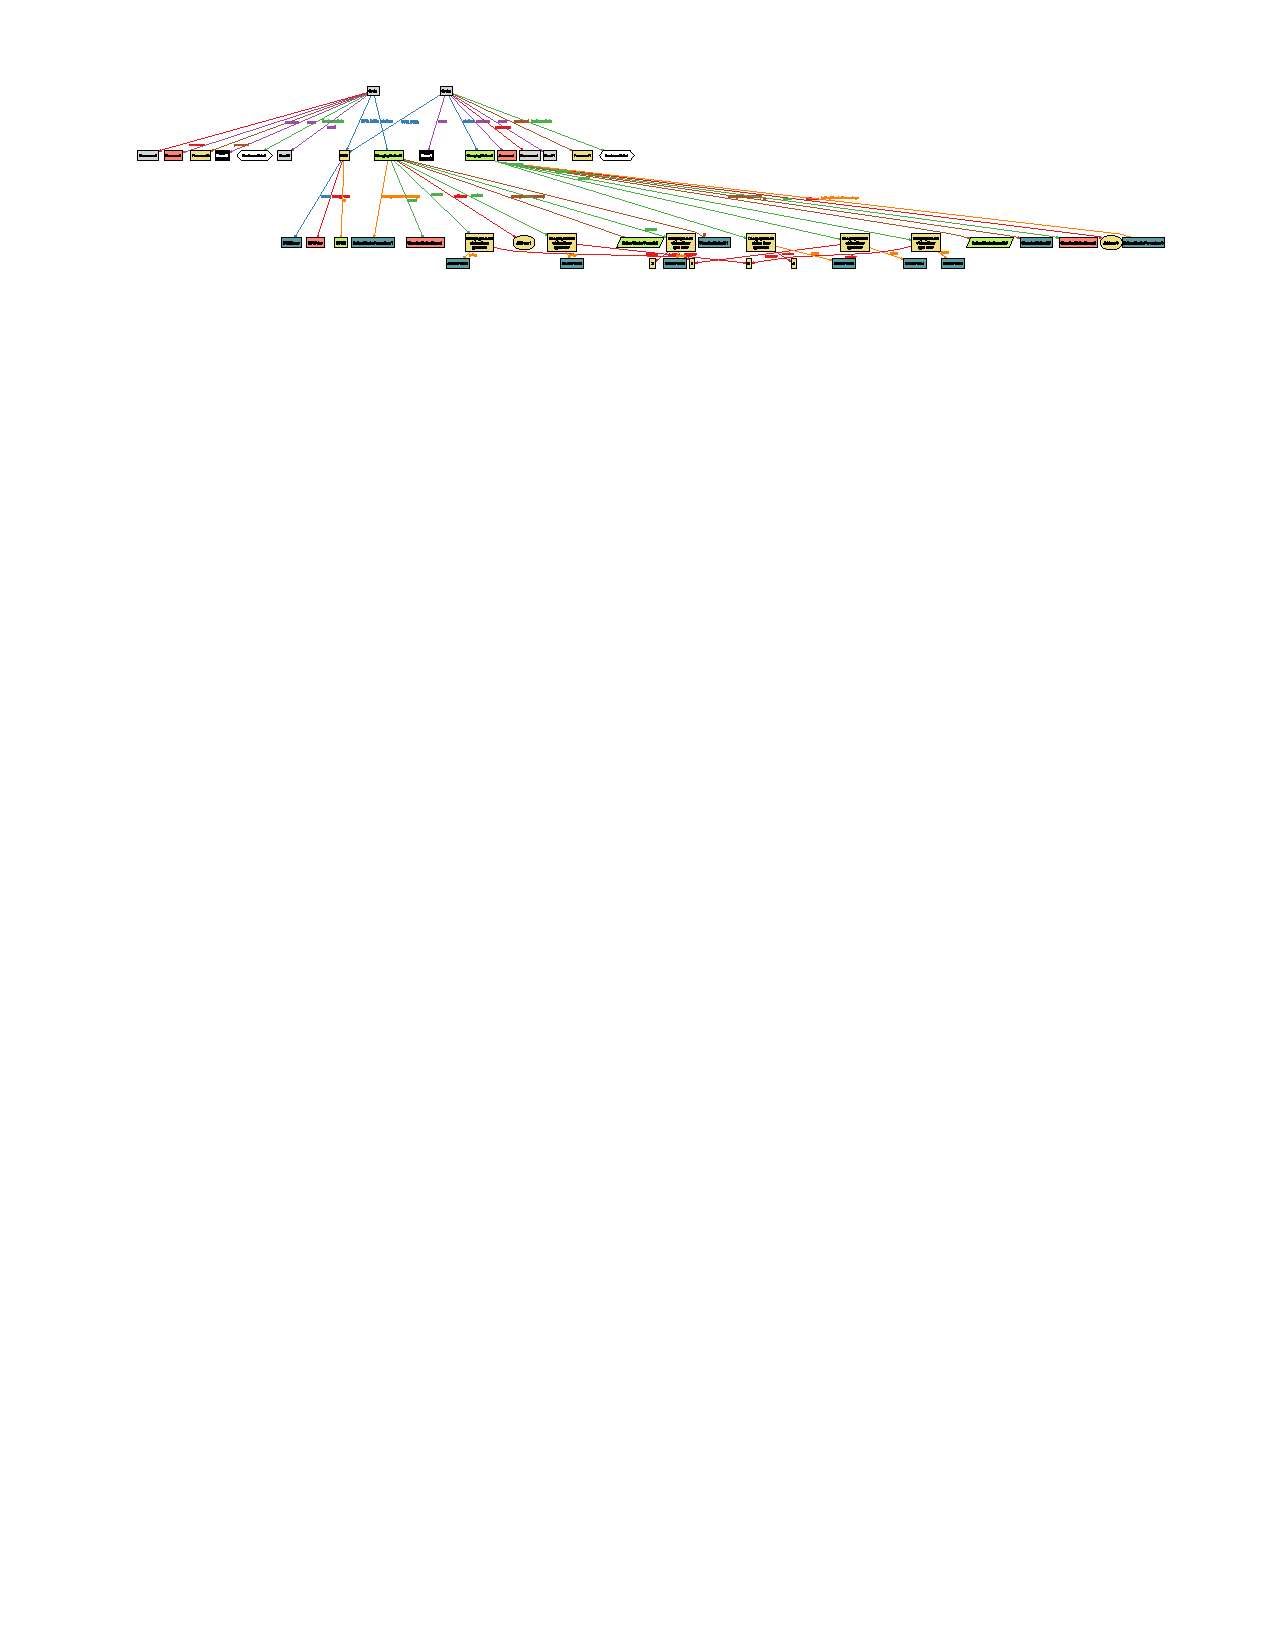
\includegraphics[angle=90,origin=c, height=0.85\textwidth]{images/world2.pdf}
\caption{World 2}
\label{fig:world_2}
\end{figure}
\section{First World}
The goal of the first world in the figure \ref{fig:world_1} consists in representing the booking function: the valid booking functions are then displayed relating to a charging station which contains a charging socket (which can be busy or free and fast, slow or rapid).\\
It is important to note that the bookings made for the same day are not overlapping in terms of timeslots.
\section{Second World}
The goal of the second world in the figure \ref{fig:world_2} is to represent the structure of the charging stations and related charging sockets, paying particular attention to the fact that there are no identical charging socket codes in the same charging stations.